%=========================================%
%-->    Lab: Two RLC Resonant Circuits <--%
%--> Author: Charles Edward Pax        <--%
%-->   Date: 2006.02.07                <--%
%=========================================%
%
%
\documentclass[11pt,onecolumn]{article}
\usepackage{color,graphics}
\begin{document}
\title{Two RLC Resonant Circuits}
\date{\today}
\author{Charles Edward Pax}
\maketitle

%=====================%
%--> Sec: Abstract <--%
%=====================%
\abstract{This report describes the frequency response of both parallel and series RLC circuits using both sinsusoidal and square wave inputs. Resonance, the notch effect, and ringing are discussed.}

%=========================%
%--> Sec: Introduction <--%
%=========================%
\section{Introduction}\label{sec:Introduction}
Circuits composed of resistors, inductors, and capacitors (RLC) resonate when the components are in parallel or in series and operating under a sinusoidal input. Both parallel and series RLC circuits can be used as filters and their frequency responses used to help understand the behavior of the RLC circuit.

Such a circuit can be used as a notch filter. The notch frequency  $\omega_0$ is defined as the frequency for which the circuit's transfer function is purely real\cite{Electric_Circuits}. For both series and parallel circuits this frequency can be calculated using equation \ref{eq:notch_frequency}.
%%
%% Notch equation
%%
\begin{equation}\label{eq:notch_frequency}
\omega_0 = \sqrt{\frac{1}{L C}}
\end{equation}

The bandwidth $\beta$ is defined as the difference between the two cutoff frequencies, which are defined by equations \ref{eq:omega_c1} and \ref{eq:omega_c2}\cite{Electric_Circuits}.
%%
%% Cutoff frequencies
%%
\begin{equation}\label{eq:omega_c1}
\omega_{c1} = -\frac{R}{2L} + \sqrt{\left( \frac{R}{2L} \right)^2 + \left( \frac{1}{L C} \right)}
\end{equation}
\begin{equation}\label{eq:omega_c2}
\omega_{c2} = \frac{R}{2L} + \sqrt{\left( \frac{R}{2L} \right)^2 + \left( \frac{1}{L C} \right)}
\end{equation}

%=================%
%--> Sec: Data <--%
%=================%
\section{Data}\label{sec:Data}
\subsection{Part A}
A notch filter was constructed using an inductor ($L$ = 1 mH) in parallel witha capacitor ($C$ = 0.1 $\mu$F), and the pair in series with a resistor ($R$ = 1 k$\Omega$) as seen in figure \ref{fig:Notch_Filter}.
%%
%% Notch filter diagram
%%
\begin{figure}
\begin{center}
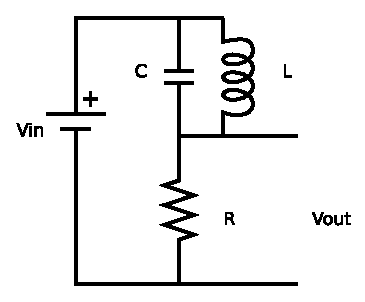
\includegraphics{Diagram1.eps}
\end{center}
\caption{Notch filter with two components in parallel.}\label{fig:Notch_Filter}
\end{figure}

Measurements for $V_{out}$ were taken at various sinusoidal driving voltage frequencies ranging from 100 Hz to 1 MHz with relevant measurements plotted in figure \ref{fig:plot01}. The measurements were repeated with $R$ = 100 $\Omega$ and plotted in figure \ref{fig:plot02}.
%%
%% Experimental data
%%
\begin{figure}
\begin{center}
\input{plot01}
\end{center}
\caption{Notch frequency for a capacitor ($C$ = 0.1 $\mu$F) in parallel with an inductor ($L$ = 1 mH), in series with a resistor ($R$ = 1 k$\Omega$).}\label{fig:plot01}
\end{figure}
%%
%% Experimental data
%%
\begin{figure}
\begin{center}
\input{plot02}
\end{center}
\caption{Notch frequency for a capacitor ($C$ = 0.1 $\mu$F) in parallel with an inductor ($L$ = 1 mH), in series with a resistor ($R$ = 100 $\Omega$).}\label{fig:plot02}
\end{figure}

The response of the circuit to a low-frequency square-wave input was observed to be that of {\em ringing} on the oscilloscope. Estimates of the values displayed on the oscilloscope screen were recorded and are plotted in figure \ref{fig:Ringing}\footnote{Answer to question 3.}.
%%
%% Ringing
%%
\begin{figure}
\begin{center}
\input{plot03}
\end{center}
\caption{Ringing. Data is an estimate of the image displayed on the oscilloscope screen.}\label{fig:Ringing}
\end{figure}

%%
%% Part B
%%
\subsection{Part B}
A notch filter was constructed using an inductor ($L$ = 1 mH) in parallel witha capacitor ($C$ = 0.1 $\mu$F), and the pair in series with a resistor ($R$ = 100 $\Omega$) as seen in figure \ref{fig:Notch_Filter_series}.
\begin{figure}
\begin{center}
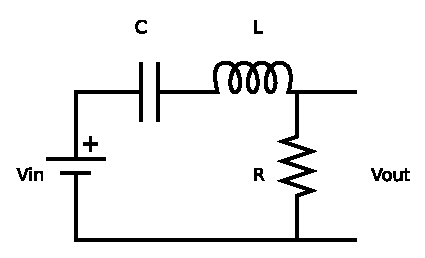
\includegraphics{Diagram2.eps}
\end{center}
\caption{Notch filter with all components in series.}\label{fig:Notch_Filter_series}
\end{figure}

%==================================%
%--> Sec: Discussion & Analysis <--%
%==================================%
\section{Discussion \& Analysis}\label{sec:Discussion}
\subsection{Part A}\label{sec:Part_A}
The notch frequency for the circuit in figure \ref{fig:Notch_Filter} is calculated using equation \ref{eq:notch_frequency},
\begin{displaymath}
\omega_0 = \sqrt{\frac{1}{L C}} = \sqrt{\frac{1}{0.001\ \mathrm{H} \cdot 0.00000001 \mu \mathrm{F}}} = 100\ \mathrm{kHz}
\end{displaymath}
This differs by 80 kHz from our experimental value of approximatly 20 kHz for both $R$ = 1 k$\Omega$ and $R$ = 100 $\Omega$. Though our calculated and experimental values for $\omega_0$ differ greatly, the readings demonstrate that $\omega_0$ is independent of the resistance of $R$.

For the circuit in figure \ref{fig:Notch_Filter}, where $R$ = 1 k$\Omega$, equations \ref{eq:omega_c1} and \ref{eq:omega_c2} are used to find the bandwidth,
\begin{displaymath}
\beta = \omega_{c2} - \omega_{c1} = 1009901.95 - 9901.95 = 1\ \mathrm{MHz}
\end{displaymath}
and for $R$ = 100 $\Omega$,
\begin{displaymath}
\beta = \omega_{c2} - \omega_{c1} = 161803 - 61803 = 100\ \mathrm{kHz}
\end{displaymath}
Again, the measured and experimental values differ greatly. However, figures \ref{fig:plot01} and \ref{fig:plot02} clearly demonstrate the bandwidth dependence the resistance of $R$ by the visable widths the portion or each graph where the $V_{out}$ drops sharply\footnote{Answer to question 1.}.

The differences observed in figures \ref{fig:plot01} and \ref{fig:plot02} make sense because equation \ref{eq:notch_frequency} shows the notch frequency to be dependent only on $L$ and $C$ while equations \ref{eq:omega_c1} and \ref{eq:omega_c2} show the bandwidth to also be dependent on $R$\footnote{Answer to question 2.}.

For the ringing observed in figure \ref{fig:Ringing}, the wavelength must be estimated by multiplying the time from the anti-peak to the peak by two. This gives a frequency of 20 kHz.
\begin{displaymath}
\omega = \frac{1}{\lambda} = \frac{1}{2 (0.000035 - 0.000010)} = 20\ \mathrm{kHz}
\end{displaymath}

\subsection{Part B}
The impedance for the circuit in figure \ref{fig:Notch_Filter_series} is the sum of the impedances of its components\footnote{Answer to question 6.}.
\begin{displaymath}
Z = \frac{-j}{\omega}C + j \omega L + R = 100 - 480 j = 100\ \mathrm{Ohm}
\end{displaymath}


%========================%
%--> Sec: Conclusions <--%
%========================%
\section{Conclusions}\label{sec:Conclusions}
The experimental values well exceed a reasonable deviation from the calculated values and demonstrate a large systematic error. The capacitor or inductor used is likely to have been different than what it was believed to be. This is an error on the part of the experimentor, but does not affect the conclusions that the notch frequency $\omega_0$ is independent of resistor $R$ and bandwidth is dependent on resistor $R$.

In the calculations for bandwidth in section \ref{sec:Part_A} appear to be the opposite of what is expected. The incorrect resistros may have been used.

As  $R$ was increased from 100 $\Omega$ to 1 k$\Omega$ to 10 k$\Omega$, the amount of decay decreased. The wave form for more values of $R$ would have to be observed to make a comprehensive statement, however, it appears that the amount of dampening of the wave is dependent on the resistance of $R$\footnote{Answer to question 4.}.

%=========================%
%--> Sec: Bibliography <--%
%=========================%
\begin{thebibliography}{9}
\bibitem{Electric_Circuits} James W. Nilsson, Susan A. Riedel, {\em Electric Circuits}, 6$^{th}$ edition, 2001, ISBN: 0-13-032120-6.
\end{thebibliography}

\end{document}
